\chapter{Coding}

This is an test lab to help you debug and verify your pipeline.  At the moment you don't have a hazard detection circuit to do a stall/slip or a forwarding unit to pass values to where they are needed so you will need to put four no-ops between each real instruction to ensure everything finishes.  If you have time you can implement forwarding at the end of the lab and earn extra credit!

\section{Implementing Code}
Pick a snipet of MIPS code that you know how it works and what it will produce from the text or one of my sample tests.  Copy the three sum testfiles and rename them to put your machine code in.  Assemble each line of your chosen snipet into MIPS machine code and replace the instructions (not the no-ops) in the files.  Specify the starting data values in the registers and data memory by changing the contents of your newly renamed R and D files.  Change the file names pointed to in the `definitions.vh' file to the new ones.  Run your simulation and verify the functioning of the code!  I suggest each partner pick one snipet to do, so you will get two verifications.

\section{Forwarding}
If you finished the pipeline and verified it successfully then congratulations you hit a great milestone!  Now see if you can modify the pipeline you built to include the forwarding unit in Fig~\ref{fig:forwarding}.  This will allow R-Type commands to go back to back, i.e. no four command delay between them.  

\textbf{Make a copy of your project and call the new one forwarding or something.}  Many people have ruined their project and not had an easy way to restart, please be careful.
  
Go one step at a time and implement everything in the picture.  The components are simple, so I don't think you should have a problem. You will need to make new wires and break old connections.  You will also have to add ports to your existing modules.  I suggest picking a direction - inside out or outside it - meaning start from inside the lowest level module in a stage and work out till the stage is done, or work from the interface of the stage to the lowest level module (outside in).  Either is fine, one will fit your style better. 

If you finish it, write it up and name it `LabForwarding' so I can find it easily.  You have now hit the ultra elite group of about the top 10\% of all computer organization students I have taught.  Great job!

\begin{figure}
\caption{Pipeline with forwarding.}\label{fig:forwarding}
\begin{center}
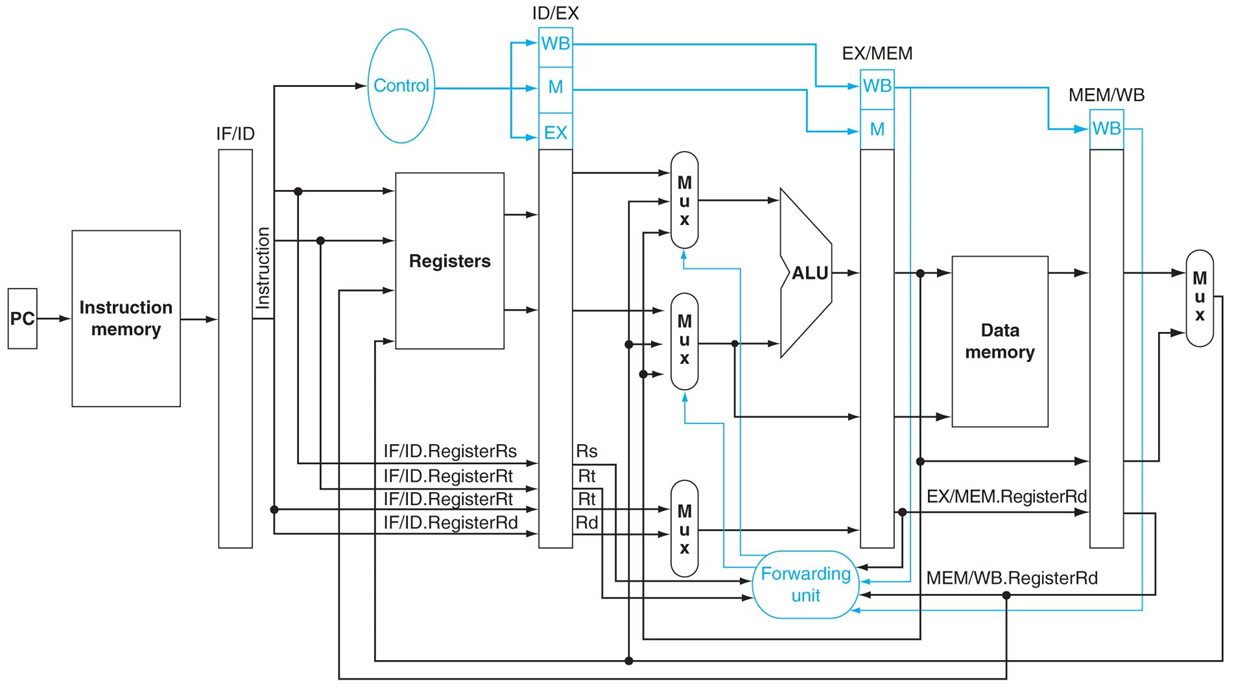
\includegraphics[width=\textwidth]{../images/pipeline_forward.png}
\end{center}
\end{figure}

\section{Your Assignment}

You are to:
\begin{enumerate}
\item Finish your pipeline if not done.
\item Each partner should convert a snipet of code, run it, and verify the solution.
\item Write up a lab report in \LaTeX\ following the lab format in \verb1LabN.tex1 and generate a pdf file.
\item Upload the pdf and all the Verilog files to the course LMS.
\end{enumerate} 

\noindent
For extra credit you can:
\begin{enumerate}
\item Add forwarding, then run a simulation and generate a timing diagram to verify.
\item Write up a lab report in \LaTeX\ following the lab format in \verb1LabN.tex1 and generate a pdf file as `LabForwarding.pdf'.
\item Upload the pdf and a zip of all the Verilog files for forwarding (to keep the separate) to the course LMS.
\end{enumerate} 

